\section{System Design}

The system of the validator nodes and their supporting components are designed to provide security and stability. The basic layout is shown in Figure ~\ref{fig:sysdesign}.

\begin{figure}[ht]
	\centering
    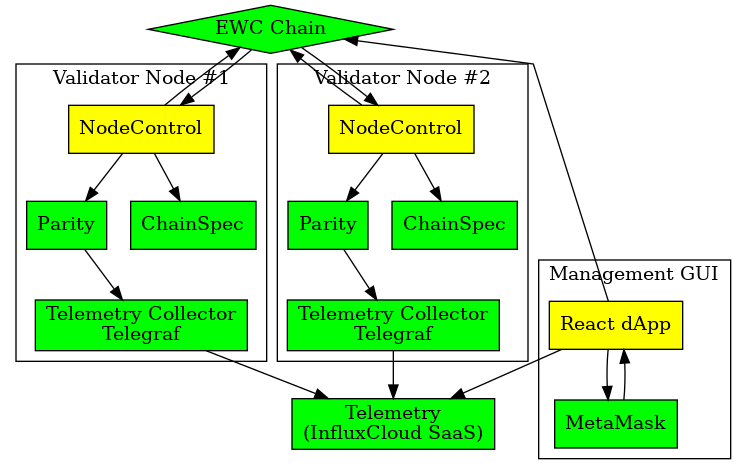
\includegraphics[width=0.85\textwidth,keepaspectratio]{./images/sys-diagram.png}
	\caption{Validator System Design}
	\label{fig:sysdesign}
\end{figure}

\subsection{System Components}
\label{components}

These system components are tailor made or where developed for the validator network.

\subsubsection{NodeControl}

A small deamon that will carry out updates on behalf of NetOps. See \ref{nodecontrol}.

\subsection{Other Components}

These components are standardize open-source components.

\subsubsection{Telemetry Collector}

The system uses Telegraf to collect the telemetry from on the nodes. This collected data is then send via the InfluxDB wire protocol to the also locally running telemetry signer.

\subsubsection{Telemetry SaaS Backend}

To gather and visualize the telemetry a SaaS provider is used.

\subsubsection{Blockchain Client}

The blockchain client is the main component of the system as it provides the connection to the blockchain and also carries out signing and validation duties. 
The probably used software will be Parity-Ethereum from Parity Tech running the AURA Proof-of-Authority engine.

